\section{Эксперимент}
\section{Часть}
\begin{equation} 
    CuSO_4 + 2NaOH \xrightarrow{}  Cu(OH)_2 + Na_2SO_4
\end{equation} 
\begin{equation} 
    CoCl_2 + 2NaOH \xrightarrow{} Co(OH)2 + 2NaCl
\end{equation} 
Это реакции осаждения в ходе котрой образовалось растоворимое 
вещество. Поэтому растоворы данных рекций прозрачны.

\begin{figure}[h]
    \centering
    \begin{subfigure}[b]{0.45\textwidth}
    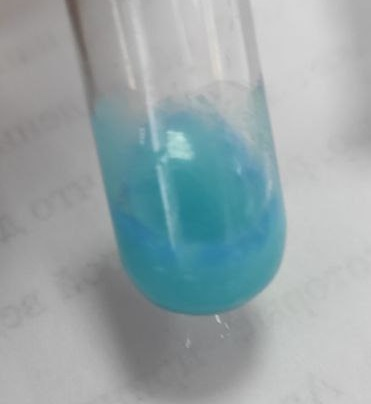
\includegraphics[width=\textwidth]{Ex_5/Cu_1.jpg}
    \caption{$Cu(OH)_2 + Na_2SO_4$}
    \end{subfigure}
    \quad
    \begin{subfigure}[b]{0.45\textwidth}
    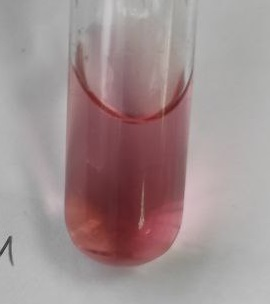
\includegraphics[width=\textwidth]{Ex_5/Co_1.jpg}
    \caption{$Co(OH)_2 + 2NaCl$}
    \end{subfigure}
    \caption{Реакции первого этапа с $CoCl_2 \land CuSO_4$}
\end{figure}

Соединяем с раствором аммиака.
\begin{equation}
    CoCl_2 + 2NaOH + 2NH_3 \xrightarrow{} Co(OH)_2 \downarrow + 2NaCl + 2NH_4Cl
\end{equation}
\begin{equation}
    Cu(OH)_2 + Na_2SO_4 + 4NH_3 \xrightarrow{} Cu(NH_3)_4 + H_2O + Na_2O + SO_4
\end{equation}

\begin{figure}[h]
    \centering
    \begin{subfigure}[b]{0.45\textwidth}
    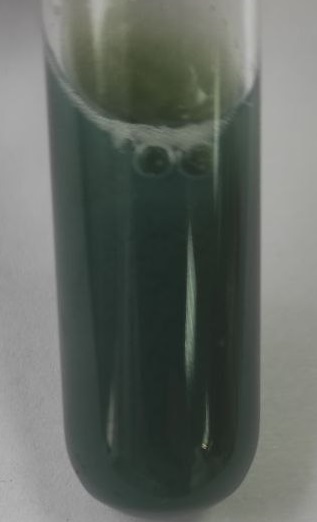
\includegraphics[width=\textwidth]{Ex_5/Cu_2.jpg}
    \caption{$Cu(OH)_2 + Na_2SO_4$}
    \end{subfigure}
    \quad
    \begin{subfigure}[b]{0.45\textwidth}
    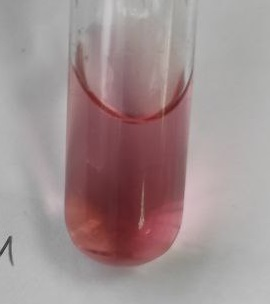
\includegraphics[width=\textwidth]{Ex_5/Co_1.jpg}
    \caption{$Co(OH)_2 + 2NaCl$}
    \end{subfigure}
    \caption{Реакции первого этапа с $CoCl_2 \land CuSO_4$}
\end{figure}


\section{Часть}



    

